\chapter{Algorithm configuration}
\label{ch:Algorithm configuration}
Many of the methods proposed in chapter \ref{ch:Analysis of the pattern recognition problem} require \emph{hyper-parameters}.  A hyper-parameter is a setting parameter that varies aspects of the algorithm and might lead to better or worse results.To ensure that all the algorithms are comparable with each other this chapter goes over the process of finding the optimal hyper-parameters for every approach. In the process a f\textsubscript{2}-score is assigned to every algorithm under the condition of optimal hyper-parameters.
\section*{Hyper-parameter tuning}
The process of searching and finding good hyper-parameters for a given algorithm is called \emph{hyper-parameter tuning}. Searching for good hyper parameters takes the following aspects to be considered:
\begin{itemize}
\item{ \textbf{an estimator}} \\
The  \emph{estimator} in this case is a binary classifier. The 8 different binary classifiers have to be considered as mentioned in chapter \ref{ch:Analysis of the pattern recognition problem}.
\item{\textbf{a parameter space}} \\
The  \emph{parameter space} defines a set of parameters or combination of parameters that will be tested. From this set one element will be chosen as most fitting. Because every algorithm requires different parameters, the parameter space is different for every algorithm. The parameter space will be defined in the sections below for every algorithm. 
\item{\textbf{a method for searching or sampling candidates}}\\
The method that is chosen is grid search. Grid search is a brute force search, which uses an exhaustive searching through a defined parameter space. Models and iteratively trained and evaluated by a score function. The model scores are then compared. The hyper-parameters that produced the best performing model will be chosen as optimal ones for the algorithm.
\item{\textbf{a cross-validation scheme}} \\
The  \emph{cross-validation scheme} used is a k-fold validation, with k=10.
\item{\textbf{a score function}}\\
As mentioned in chapter \ref{ch:Analysis of the pattern recognition problem}  a  f\textsubscript{2}-score will be used to evaluate the models in the end. Our goal for the hyper-parameter tuning is thereby also to maximise the  f\textsubscript{2}-score. For that reason the  f\textsubscript{2}-score is used as a score function.
\end{itemize}

For the hyper-parameter search no external functions or libraries are used. The search algorithm is implemented in the following way.\\ For the given estimator (one of the possible classification algorithms) the parameter space is defined manually for every hyper-parameter.\\
Models are now repeatedly trained by iterating through every combination of hyper-parameters in the parameter spaces.\\
For every trained model a  k-fold validation, with k=10, is performed.\\
During the k-fold validation, the f\textsubscript{2}-score is calculated.\\
After this process is done the hyper-parameters that resulted in the highest f\textsubscript{2}-score are chosen.\\
In the following for each of the relevant algorithms a parameter space will be defined. The results of the hyper parameter search will then be presented.

\subsection*{Linear SVM}
The tunable hyper-parameters for the the linear SVM classifier is the regularization. \\
\textbf{L1 regularization:}\\
$\sum_{i=1}^{n}|y\textsubscript{i}-f(x\textsubscript{i})| $ \\
 y\textsubscript{i} is the target value and x\textsubscript{i} is the estimated value for y\textsubscript{i}.\\
 L1 regularization is a loss function that minimizes the sum of the absolute differences of target and estimated value.
\\
\textbf{L2 regularization:}  \\
$\sum_{i=1}^{n}(y\textsubscript{i}-f(x\textsubscript{i}))^2 $ \\
 y\textsubscript{i} is the target value and x\textsubscript{i} is the estimated value for  y\textsubscript{i}.\\
 L2 regularization is a loss function that minimizes the square of the absolute differences of target and estimated value.
\\

The hyper-parameter search reveals the following results for the two regularization approaches: \\

\pgfplotsset{width=1.1\textwidth, height=0.5\textwidth}

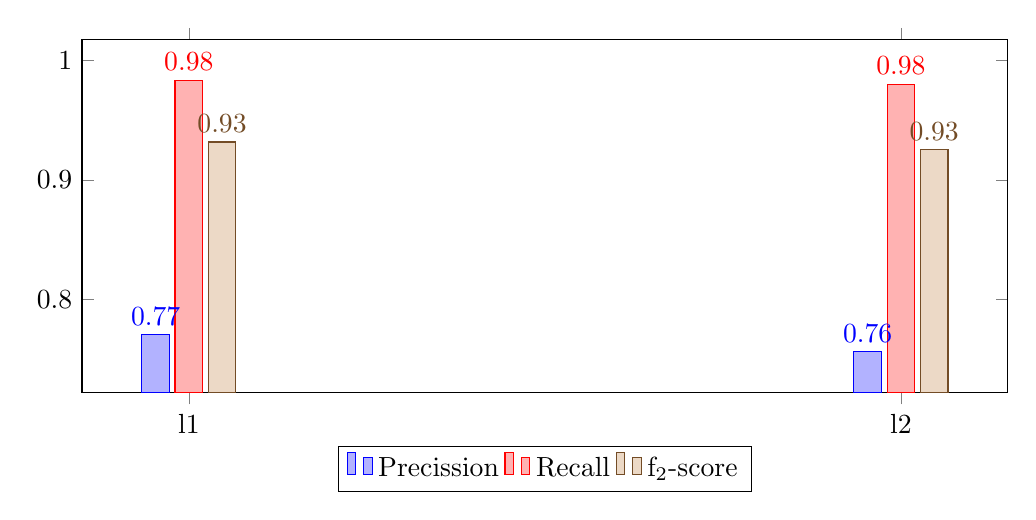
\begin{tikzpicture}
\begin{axis}[
ybar,
enlargelimits=0.15,
legend style={at={(0.5,-0.15)},
anchor=north,legend columns=-1},
xlabel={Regularization},
symbolic x coords={l1,l2},
xtick=data,
nodes near coords,
nodes near coords align={vertical},
]
\addplot coordinates {(l1,0.770476190476)(l2,0.75619047619)};

\addplot coordinates {(l1,0.983333333333)(l2,0.98)};

\addplot coordinates {(l1,0.931845691305)(l2,0.925231866825)};

\legend{Precission, Recall, f\textsubscript{2}-score}
\end{axis} 
\end{tikzpicture}
\\


The best performing SVM model reaches a maximal {f\textsubscript{2}-score of \textbf{0.93} (precision:  0.77, recall: 0.98) with the following hyper-parameter:\\
Regularization: \qquad  \qquad \textbf{l1 regularization}

\subsection*{Logistic regression}
The tunable hyper-parameters for the the logistic regression classifier is the regularization. 
\\
\textbf{L1 regularization:}\\
$\sum_{i=1}^{n}|y\textsubscript{i}-f(x\textsubscript{i})| $ \\
 y\textsubscript{i} is the target value and x\textsubscript{i} is the estimated value for y\textsubscript{i}.\\
 L1 regularization is a loss function that minimizes the sum of the absolute differences of target and estimated value.
\\
\textbf{L2 regularization:}  \\
$\sum_{i=1}^{n}(y\textsubscript{i}-f(x\textsubscript{i}))^2 $ \\
 y\textsubscript{i} is the target value and x\textsubscript{i} is the estimated value for y\textsubscript{i}.\\
 L2 regularization is a loss function that minimizes the square of the absolute differences of target and estimated value.
\\

The hyper-parameter search reveals the following results for the two regularization approaches: \\

\pgfplotsset{width=1.1\textwidth, height=0.5\textwidth}

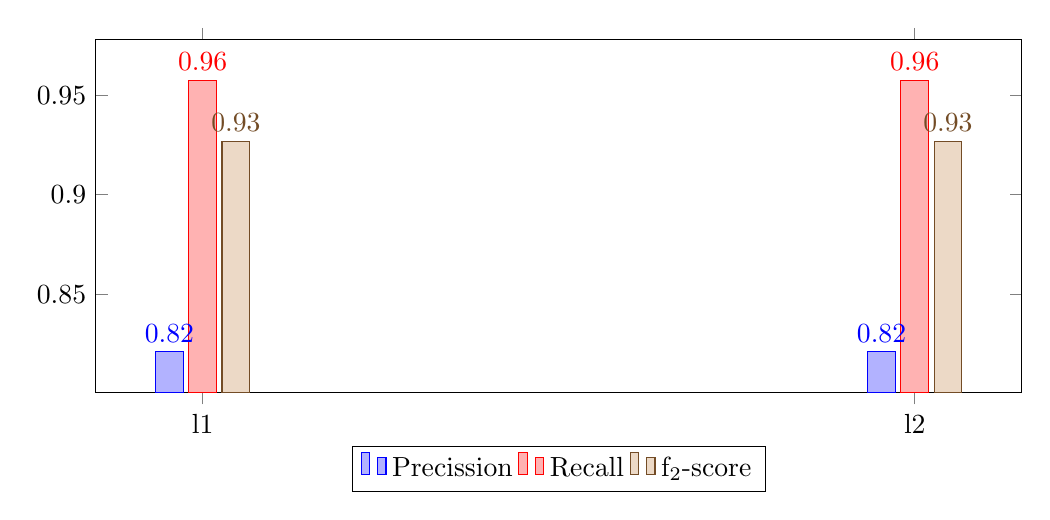
\begin{tikzpicture}
\begin{axis}[
ybar,
enlargelimits=0.15,
legend style={at={(0.5,-0.15)},
anchor=north,legend columns=-1},
xlabel={Regularization},
symbolic x coords={l1,l2},
xtick=data,
nodes near coords,
nodes near coords align={vertical},
]
\addplot coordinates {(l1,0.820952380952)(l2,0.820952380952)};

\addplot coordinates {(l1, 0.9575)(l2, 0.9575)};

\addplot coordinates {(l1,0.926673590255)(l2,0.926673590255)};

\legend{Precission, Recall, f\textsubscript{2}-score}
\end{axis} 
\end{tikzpicture}
\\


The best performing logistic regression model reaches a maximal {f\textsubscript{2}-score of \textbf{0.93} (precision:  0.82, recall:0.95) independent of which regularization is used.

\subsection*{Decision tree}
The tunable hyper-parameters for the decision tree algorithm are:
\begin{itemize}
\item{\textbf{Impurity}}\\
The impurity measure is used to decide on a splitting rule for each node in the decision tree building process.
Two impurity measures for classification are provided:\\
\textbf{Gini impurity:}  \\
$\sum_{i=1}^{C} f\textsubscript{i}(1-f\textsubscript{i}) $ \\
C is the number of unique labels and f\textsubscript{i} is the frequency of label i in a node. \\
\textbf{Entropy:}\\
$\frac{1}{N}\sum_{i=1}^{C} -f\textsubscript{i}\log(f\textsubscript{i}) $ \\
C is the number of unique labels and f\textsubscript{i} is the frequency of label i in a node. \\
\item{\textbf{Maximal depth}}\\
The maximal depth determines a limit of growth for a decision tree. This consequentially limits the number of nodes or decisions that are possible. It represents a stopping criteria. \\
The parameter space for the maximal depth is chosen \textbf{from 1 to 10} (inclusive). 
\end{itemize}

The hyper-parameter search reveals the following results: \\

\pgfplotsset{width=1.1\textwidth, height=0.5\textwidth}

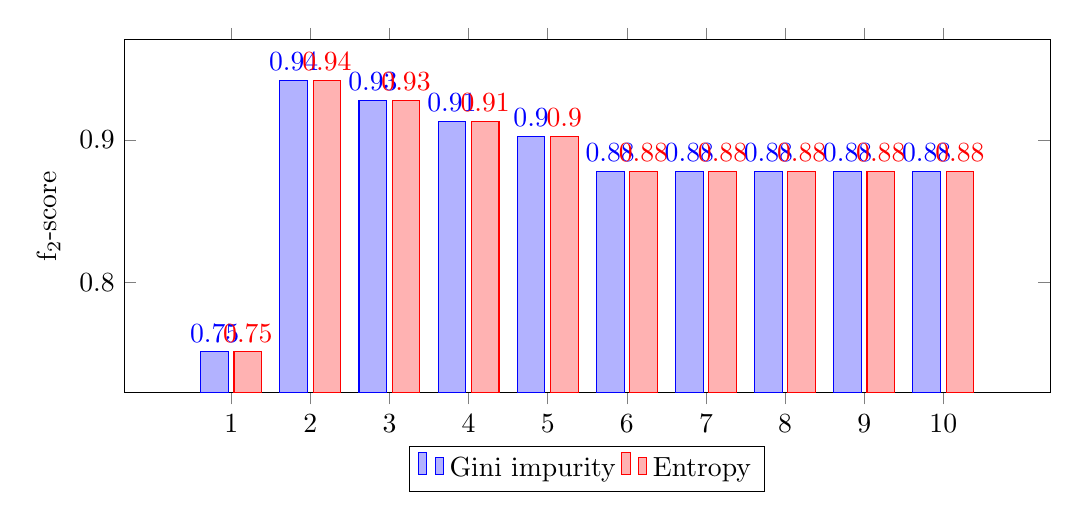
\begin{tikzpicture}
\begin{axis}[
ybar,
enlargelimits=0.15,
legend style={at={(0.5,-0.15)},
anchor=north,legend columns=-1},
xlabel={Maximal depth},
ylabel={f\textsubscript{2}-score},
symbolic x coords={1,2,3,4,5,6,7,8,9,10},
xtick=data,
nodes near coords,
nodes near coords align={vertical},
]
\addplot coordinates {(1, 0.7514765369250439)	(2, 0.94167516977742205)	(3, 0.92745939539660371)	(4, 0.91277351764611503)	(5, 0.90267105713062501)	(6, 0.87786051720271308)	(7, 0.87786051720271308)	(8, 0.87786051720271308)	(9, 0.87786051720271308)	(10, 0.87786051720271308)
};

\addplot coordinates {(1, 0.7514765369250439)	(2, 0.94167516977742205)	(3, 0.92745939539660371)	(4, 0.91277351764611503)	(5, 0.90267105713062501)	(6, 0.87786051720271308)	(7, 0.87786051720271308)	(8, 0.87786051720271308)	(9, 0.87786051720271308)	(10, 0.87786051720271308)
};
\legend{Gini impurity,Entropy}
\end{axis} 
\end{tikzpicture}
\\
The best performing decision tree model reaches a maximal {f\textsubscript{2}-score of \textbf{0.94} (precision:  0.92, recall: 0.96) with the following hyper-parameters:\\
Impurity: \qquad  \qquad \textbf{Ginni Impurity} or \textbf{Entropy} \\
Maximal depth: \qquad \textbf{2}




\subsection*{Random forest}

The tunable hyper-parameters for the random forest classifier are:
\begin{itemize}

\item{\textbf{Number of trees}}\\
The number of trees that are build during the training phase to act as an ensemble of (randomized) decision trees.\\
The parameter space for the number of threes is chosen \textbf{from 2 to 10} (inclusive). 

\item{\textbf{Impurity}}\\
The impurity measure is used to decide on a splitting rule for each node in the decision tree building process.
Two impurity measures for classification are provided:\\
\textbf{Gini impurity:}  \\
$\sum_{i=1}^{C} f\textsubscript{i}(1-f\textsubscript{i}) $ \\
C is the number of unique labels and f\textsubscript{i} is the frequency of label i in a node. \\
\textbf{Entropy:}\\
$\frac{1}{N}\sum_{i=1}^{C} -f\textsubscript{i}\log(f\textsubscript{i}) $ \\
C is the number of unique labels and f\textsubscript{i} is the frequency of label i in a node. \\
\item{\textbf{Maximal depth}}\\
The maximal depth determines a limit of growth for a decision tree. This consequentially limits the number of nodes or decisions that are possible. It represents a stopping criteria. \\
The parameter space for the maximal depth is chosen \textbf{from 1 to 10} (inclusive). 
\end{itemize}

The hyper-parameter search reveals the following results: \\

\usepgfplotslibrary{colorbrewer}

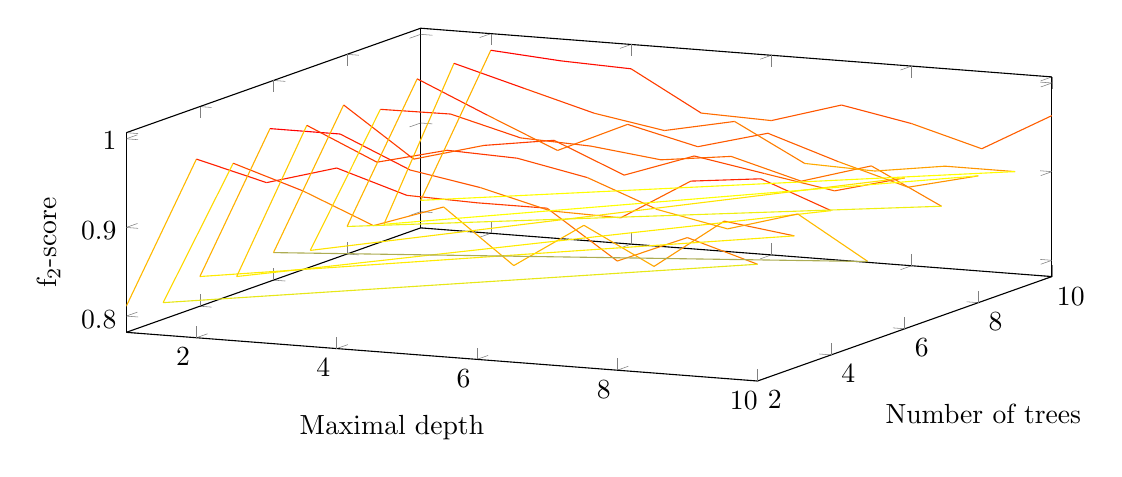
\begin{tikzpicture}
\begin{axis}[
xlabel={Maximal depth},
ylabel={Number of trees},
zlabel={f\textsubscript{2}-score}]
% this yields also a 3x4 matrix:
\addplot3 [surf] coordinates {

(1,2, 0.81117893612451164)	(2,2, 0.98319473319473327)	(3,2, 0.96274692738291667)	(4,2, 0.98534668438660011)	(5,2, 0.96059017776121025)	(6,2, 0.95830952778471323)	(7,2, 0.95830952778471323)	(8,2, 0.90483500331717981)	(9,2, 0.93734861699850558)	(10,2, 0.91339954553855851)
(1,3, 0.8004367390538728)	(2,3, 0.96378418088674134)	(3,3, 0.9384741160763842)	(4,3, 0.90561827117871407)	(5,3, 0.93275566347297345)	(6,3, 0.87275176788264619)	(7,3, 0.92428232635237662)	(8,3, 0.88400307233714881)	(9,3, 0.94119766906916114)	(10,3, 0.93067599248707811)
(1,4, 0.81514717363142675)	(2,4, 0.98811899147469606)	(3,4, 0.98811899147469606)	(4,4, 0.95358707092656092)	(5,4, 0.93986843414593968)	(6,4, 0.91975074977786109)	(7,4, 0.9180030861031705)	(8,4, 0.96551365397259359)	(9,4, 0.97421692878484434)	(10,4, 0.94439542738854887)
(1,5, 0.80043673905387258)	(2,5, 0.9770886843607306)	(3,5, 0.94161524732555246)	(4,5, 0.9611445484394654)	(5,5, 0.95830952778471323)	(6,5, 0.94255336962175351)	(7,5, 0.91256930801135139)	(8,5, 0.89691214952918386)	(9,5, 0.91980882429707833)	(10,5, 0.87226968189766674)
(1,6, 0.81270872684963535)	(2,6, 0.98534668438660011)	(3,6, 0.93032277257176865)	(4,6, 0.95190637408300693)	(5,6, 0.96378418088674134)	(6,6, 0.93059889012759778)	(7,6, 0.95830952778471323)	(8,6, 0.94459748922696507)	(9,6, 0.93116045949736315)	(10,6, 0.95190463924901969)
(1,7, 0.8004367390538728)	(2,7, 0.96566736183524504)	(3,7, 0.9664694411187349)	(4,7, 0.94563619097216911)	(5,7, 0.94251053418248987)	(6,7, 0.93314228648343533)	(7,7, 0.94310117560504569)	(8,7, 0.92122817429787718)	(9,7, 0.94459748922696507)	(10,7, 0.90517023875540015)
(1,8, 0.81270872684963535)	(2,8, 0.98534668438660011)	(3,8, 0.95049758148667896)	(4,8, 0.91672954863663902)	(5,8, 0.95231889125990454)	(6,8, 0.93319739904323273)	(7,8, 0.95448189972647135)	(8,8, 0.92868907146893775)	(9,8, 0.90581429466917407)	(10,8, 0.92474746660725948)
(1,9, 0.8004367390538728)	(2,9, 0.98811899147469606)	(3,9, 0.96599764220453888)	(4,9, 0.94402186942380006)	(5,9, 0.93059889012759778)	(6,9, 0.94697851454944548)	(7,9, 0.90569476935177529)	(8,9, 0.90323674481832927)	(9,9, 0.91480794049947445)	(10,9, 0.91480794049947445)
(1,10, 0.81270872684963535)	(2,10, 0.98811899147469606)	(3,10, 0.98226283015588589)	(4,10, 0.97941981556114444)	(5,10, 0.93558269120051019)	(6,10, 0.93319739904323273)	(7,10, 0.9568629756569883)	(8,10, 0.94201701404779536)	(9,10, 0.91975074977786109)	(10,10, 0.96323617072007628)


};
\end{axis}
\end{tikzpicture}
\\
The best performing decision tree model reaches a maximal {f\textsubscript{2}-score of \textbf{0.99} (precision:  0.94, recall: 1.0) with the following hyper-parameters:\\
Number of trees:  \qquad \textbf{4}\\
Impurity: \qquad  \qquad \textbf{Entropy} \\
Maximal depth: \qquad \textbf{2} or \textbf{3}\\
or\\
Number of trees:  \qquad \textbf{9} or \textbf{10}  \\
Impurity: \qquad  \qquad \textbf{Entropy} \\
Maximal depth: \qquad \textbf{2} 

\subsection*{Gradient-boosted trees}

The tunable hyper-parameters for the decision tree algorithm are:
\begin{itemize}
\item{\textbf{Loss function}}\\
The loss function is used for minimization during gradient boosting. The loss function provided are: \\
\textbf{LogLoss}\\
\textbf{Least Squares Error}\\
\textbf{Least Absolute Error}\\

\item{\textbf{Maximal depth}}\\
The maximal depth determines a limit of growth for a decision tree. This consequentially limits the number of nodes or decisions that are possible. It represents a stopping criteria. \\
The parameter space for the maximal depth is chosen \textbf{from 1 to 10} (inclusive). 
\end{itemize}

The hyper-parameter search reveals the following results: \\

\pgfplotsset{width=1.1\textwidth, height=0.5\textwidth}

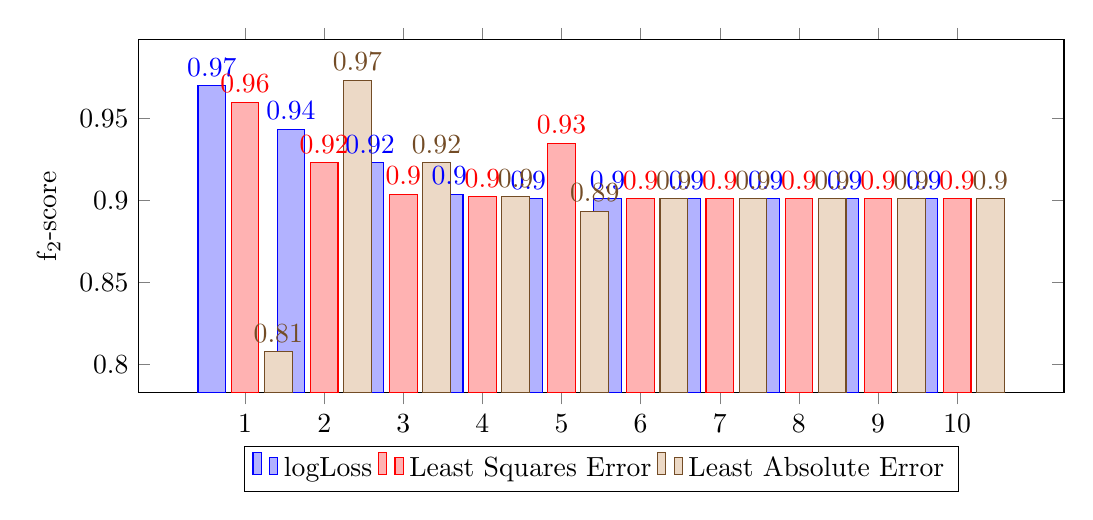
\begin{tikzpicture}
\begin{axis}[
ybar,
enlargelimits=0.15,
legend style={at={(0.5,-0.15)},
anchor=north,legend columns=-1},
xlabel={Maximal depth},
ylabel={f\textsubscript{2}-score},
symbolic x coords={1,2,3,4,5,6,7,8,9,10},
xtick=data,
nodes near coords,
nodes near coords align={vertical},
]
\addplot coordinates {
(1,0.96997949506600001 )	(2, 0.94327866731360188 )	(3, 0.92302084349494373 )	(4, 0.90371571783336502 )	(5, 0.90105794238683135 )	(6, 0.90105794238683135 )	(7, 0.90105794238683135 )	(8, 0.90105794238683135 )	(9, 0.90105794238683135 )	(10, 0.90105794238683135 )
};
\addplot coordinates {
(1, 0.95999967877678194 )	(2, 0.92302084349494373 )	(3, 0.90371571783336502 )	(4, 0.90233186341839555 )	(5, 0.93494485234132829 )	(6, 0.90105794238683135 )	(7, 0.90105794238683135 )	(8, 0.90105794238683135 )	(9, 0.90105794238683135 )	(10, 0.90105794238683135 )
};
\addplot coordinates {(1, 0.80772735483432512 )	(2, 0.97329459969909415 )	(3, 0.92302084349494373 )	(4, 0.90233186341839555 )	(5, 0.89344992226949638 )	(6, 0.90105794238683135 )	(7, 0.90105794238683135 )	(8, 0.90105794238683135 )	(9, 0.90105794238683135 )	(10, 0.90105794238683135)
};
\legend{logLoss, Least Squares Error, Least Absolute Error}
\end{axis} 
\end{tikzpicture}
\\
The best performing Gradient-boosted tree classifier reaches a maximal f\textsubscript{2}-score of \textbf{  0.97} (precision:  0.96, recall:  0.98) with the following hyper-parameters:\\
Loss function:  \qquad \textbf{Least Absolute Error}\\
Maximal depth: \qquad \textbf{2}


\subsection*{Naive Bayes}

The tunable hyper-parameters for the the Naive Bayes classifier is a $\lambda$ -value used for additive smoothing. Since the hyper-parameter search with $\lambda=[0.1,10.0]$ didn't reveal any differences in performance the hyper-parameter is not going to be regarded and will not be discussed further in this paper. \\

The naive bayes classifier reaches a f\textsubscript{2}-score of \textbf{ } (precision:  , recall: ) with the hyper-parameter:\\
$\lambda$ :  \qquad \textbf{  }\\
 